% \Image{Capa do livro (; )}{PNLD2022-016-01.png}

% \Image{Ilustração do livro (n-1 Edições/Luisa Amoroso; n-1 Edições)}{PNLD2022-016-04.png}
% \Image{Ilustração do livro (n-1 Edições/Luisa Amoroso; n-1 Edições)}{PNLD2022-016-05.png}
% \Image{Ilustração do livro (n-1 Edições/Luisa Amoroso; n-1 Edições)}{PNLD2022-016-06.png}


\documentclass[11pt]{extarticle}
\usepackage{manualdoprofessor}
\usepackage{fichatecnica}
\usepackage{lipsum,media9}
\usepackage[justification=raggedright]{caption}
\usepackage[one]{bncc}
\usepackage[lunna]{../edlab}
\usepackage{marginnote}
\usepackage{pdfpages}
\usepackage[printwatermark]{xwatermark}
\newwatermark[pagex=2]{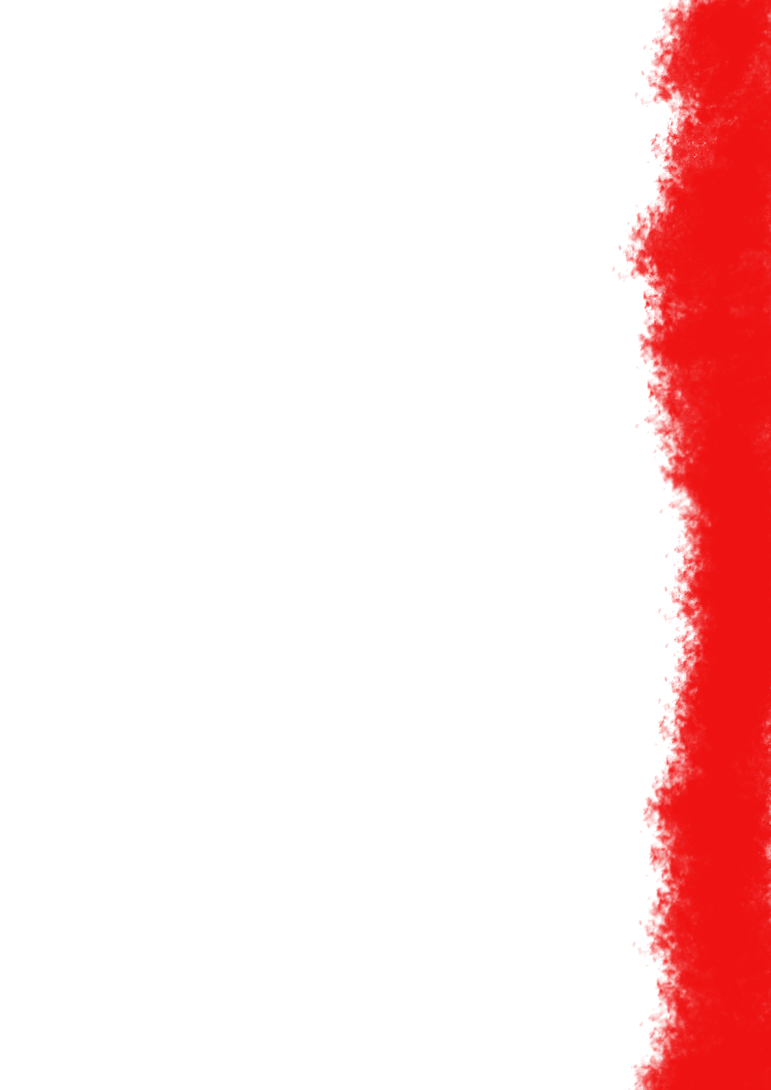
\includegraphics[scale=3.3]{watermarks/test-a.png}}	% página específica
%\newwatermark[oddpages]{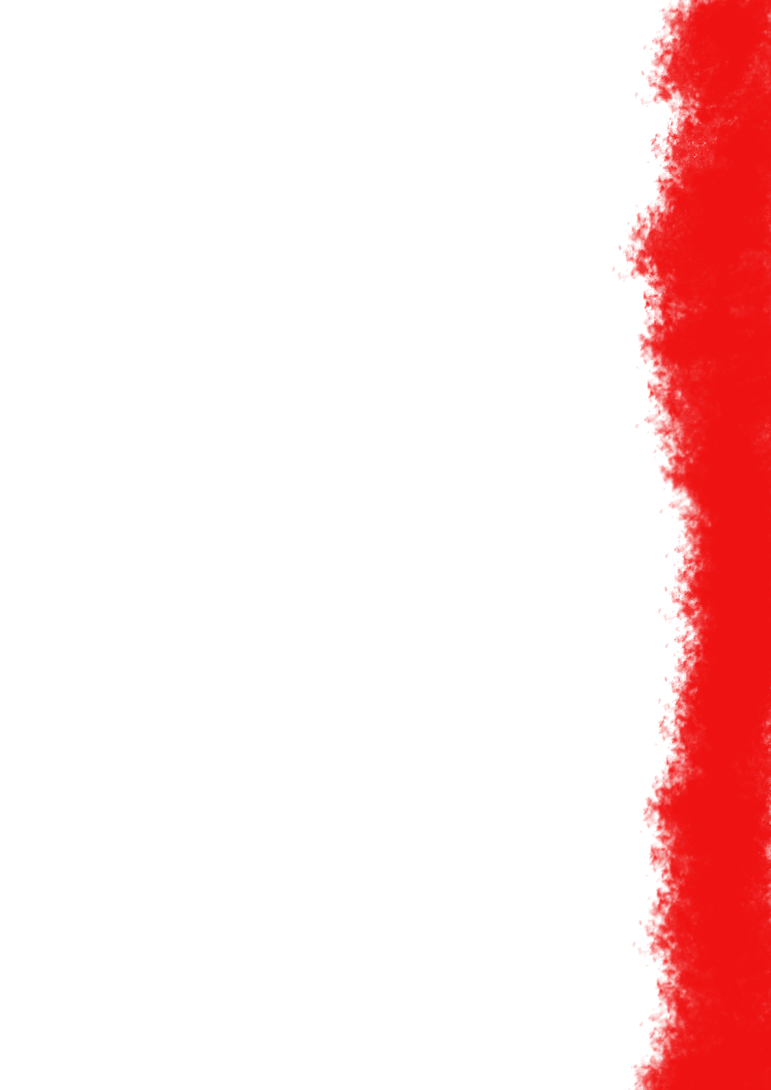
\includegraphics{watermarks/test-a.png}}			% páginas ímpars
%\newwatermark[evenpages]{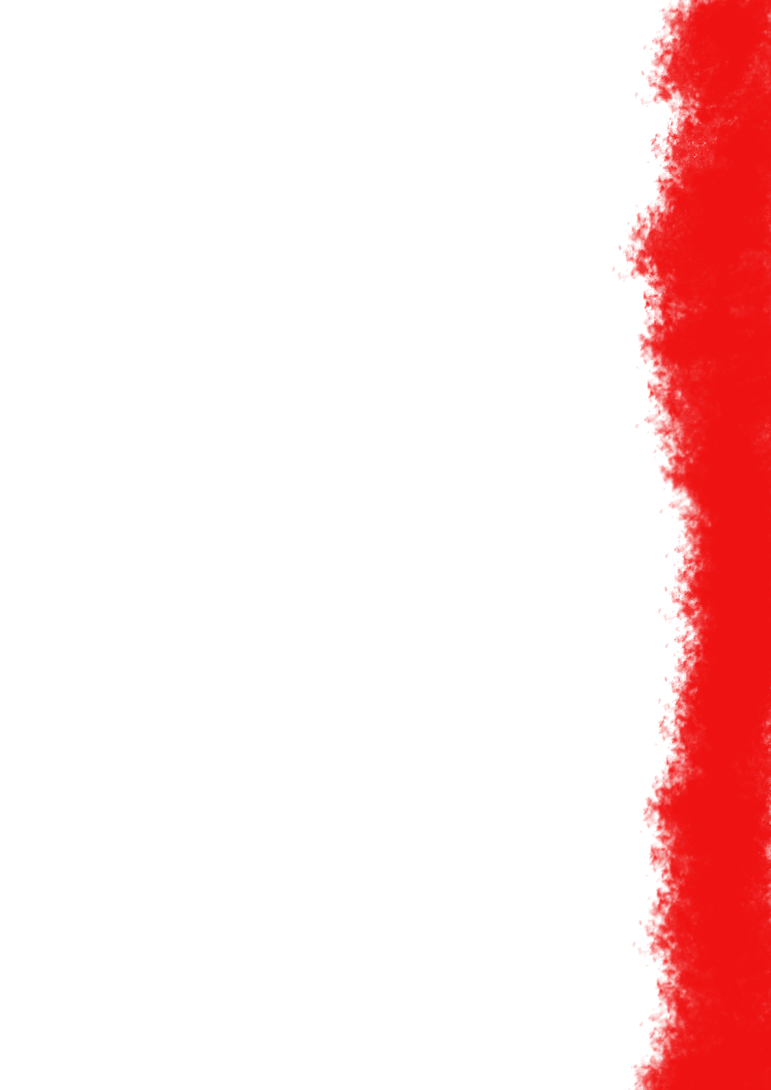
\includegraphics{watermarks/test-a.png}}			% págimas pares
\newwatermark[allpages]{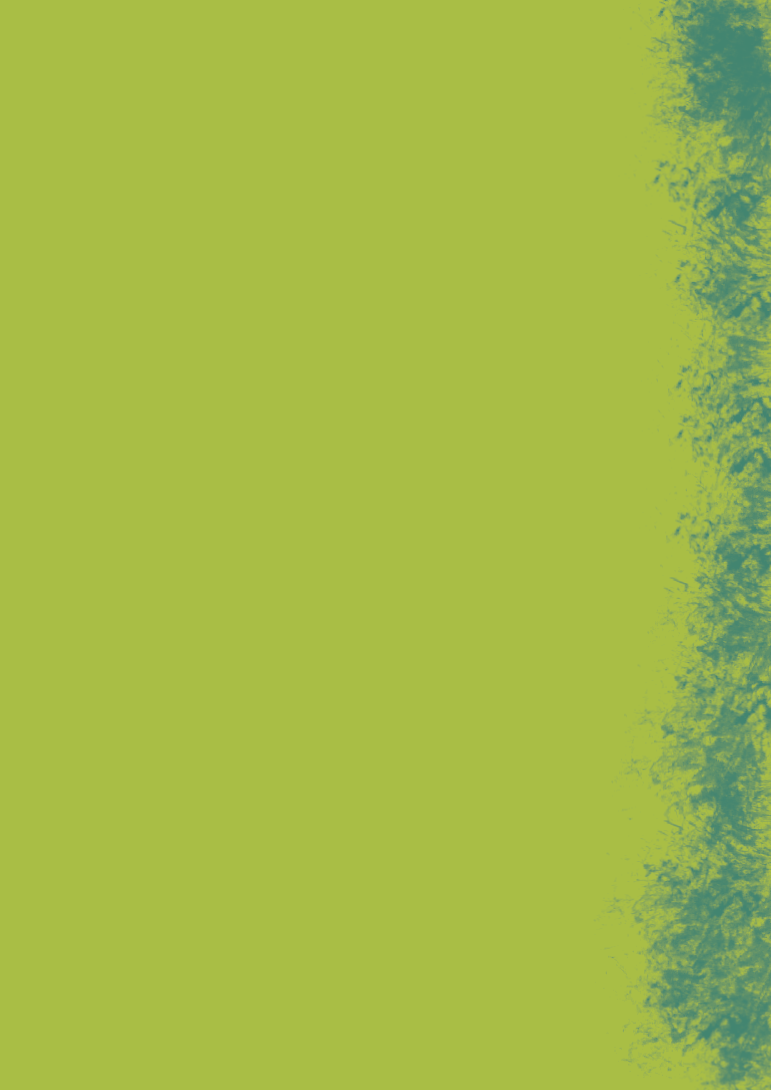
\includegraphics[scale=3.3]{watermarks/test-b.png}}
\pagecolor{cyan!0!magenta!10!yellow!28!black!28!}

\newcommand{\AutorLivro}{Uirá Garcia e Marina Magalhães}
\newcommand{\TituloLivro}{Awa rapea: caminhos dos Awá-Guajá}
\newcommand{\Tema}{Quotidiano indígena}
\newcommand{\Genero}{Prescritivos: instruções; guias; manuais; ciclo de crescimento; ciclo de vida etc}
\newcommand{\imagemCapa}{./images/PNLD2022-016-01.png}
\newcommand{\issnppub}{978-65-86941-66-1}
\newcommand{\issnepub}{978-65-86941-68-5}
% \newcommand{\fichacatalografica}{PNLD0001-00.png}
\newcommand{\colaborador}{{Paulo Pompermaier e Renier Silva}}

\begin{document}

\title{\TituloLivro}
\author{\AutorLivro}
\def\authornotes{\colaborador}

\date{}
\maketitle

%\begin{abstract}\addcontentsline{toc}{section}{Carta ao professor}
%\pagebreak

\tableofcontents



\section{Sobre o livro}

%27 caracteres
\paragraph{O livro} 
``Awa rapea: caminhos dos Awá-Guajá'' é um livro educativo com textos e imagens. 

%822 caracteres
\paragraph{Descrição} 
Preparado para ser utilizado na alfabetização do povo indígena Awá-Guajá do estado
do Maranhão, este livro apresenta o alfabeto da língua do povo, acompanhado de 
palavras referente a cada letra e uma respectiva ilustração. Tudo feito dentro do universo
cultural deles. Serão apresentados, por exemplo, a fauna e a flora locais, alguns costumes, a alimentação
etc. As ilustrações também buscam ser fieis ao imaginário local, privilegiando a 
visão que os Awá-Guajá têm dos elementos representados, e não a visão dos não indígenas. 
Junto à palavra no idioma indígena, há sua tradução em português. Isso porque 
o projeto de que o livro faz parte visa alfabetizar as pessoas nas duas línguas. 
Após a apresentação do alfabeto, há alguns textos explicativos sobre cada grupo de
palavras, dando informações culturais relevantes. Por exemplo, quais são os macacos
que são caçados e quais são domésticos, quais os efeitos da presença de máquinas
nos arredores da aldeia, e quem são os seres que vivem no céu e que regularmente
visitam a terra. 

%411 caracteres
\paragraph{Competências} 
São muitas as competências trabalhadas por este livro com os estudantes da \textbf{Pré-escola}.
A começar pela apreciação das aquarelas que ilustram as páginas que são por si só uma
obra de arte. Depois, a cada novo vocabulário e cada costume dos Awá-Guajá aprendido, 
os estudantes não indígenas são induzidos uma experiência de contato com o outro, o que eles 
já fazem nos ambientes familiar e escolar, mas desta vez, com uma intensidade maior. Os pequenos 
leitores deste livro terão a oportunidade de enriquecer seus olhares para o mundo e para as coisas
entendendo que há diferentes formas de nomear mas também de se relacionar com o mundo.
O quanto mais cedo as crianças forem solicitadas à diversidade, neste caso, dentro de
seu próprio país, mais natural para elas será o respeito e a valorização daquilo que 
é diferente. Neste sentido, este livro será um ótimo guia para a formação dos pequenos cidadãos, 
fazendo valer o Direito de Aprendizagem que diz respeito a ``conviver com outras crianças e adultos, em pequenos e grandes grupos, utilizando diferentes linguagens, ampliando o conhecimento de si e do outro, o respeito em relação à cultura e às diferenças entre as pessoas.''

%862 caracteres
\paragraph{Aprofundamento} 
Este material tem a intenção de contribuir para que você consiga desenvolver um trabalho aprofundado 
com esta obra na sala de aula. Você encontrará informações sobre o autor, sobre 
o gênero e sobre os temas trabalhados ao longo do livro. Apresentaremos também 
algumas propostas de trabalho para a sala de aula que você poderá explorar livremente, 
da forma que considerar mais apropriada para os seus estudantes. Para a prática 
da Literacia Familiar, oferecemos um guia que pode ajudar nas orientações aos 
responsáveis pela criança, para incentivar o gosto pela leitura e contribuir para 
que os estudantes desenvolvam em casa habilidades que serão importantes no momento 
da alfabetização. Por fim, você encontrará sugestões de livros, artigos e sites 
selecionados para enriquecer a sua experiência de leitura e, 
consequentemente, a de seus estudantes.


\section{Sobre o autor}

\reversemarginpar
\marginparwidth=5cm

\marginnote{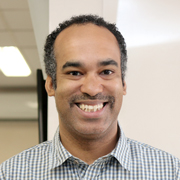
\includegraphics[width=\marginparwidth]{./images/PNLD2022-016-02.png}\\
O autor Uirá Garcia (Arquivo pessoal)}

%532 caracteres
\paragraph{O autor} 
Uirá Garcia é antropólogo e professor da Universidade Federal de São Paulo (\textsc{unifesp}). Realiza pesquisa junto aos Awá-Guajá há cerca quinze anos, onde desenvolve estudos sobre as práticas de conhecimento relativas aos animais, a caça e a floresta, tendo como foco diferentes formas de “caça”, “criação” e “manejo”, em diálogo com a etnologia indígena e a teoria antropológica de maneira geral. Os Awá são os seus grandes professores e com eles aprendeu sobre plantas, animais, e pessoas de uma maneira nova, e da importância do cuidado e atenção à floresta. 


%313 caracteres
\paragraph{Publicações} 
Além de uma extensão produção bibliográfica no meio acadêmico, Uirá Garcia é autor do livro ``Awá-Guajá: crônicas de caça e criação'' (2018/ São Paulo: Hedra).
%358 caracteres
\paragraph{Currículo} 
 Faz parte do Centro de Estudos Ameríndios (CEstA) da Universidade de São Paulo (\textsc{usp}), e do Núcleo de Antropologia Simétrica (NAnSi) do \textsc{ppgas} do Museu Nacional/\textsc{ufrj}. Foi pesquisador visitante na Universidade da Califórnia-Davis no ano de 2019.

\paragraph{A autora}
Marina Magalhães é linguista, professora da Universidade de Brasília e pesquisadora da língua falada pelos Awá-Guajá desde 2001, quando obteve a autorização para visitá-los pela primeira vez. Desde então, gradualmente foi construindo laços profissionais que foram se tornando também laços sociais e hoje tem uma parte do povo Awá como referência importante de vida. Com eles aprendeu e ver o mundo através de um prisma diferente, mais amplo, que influencia positivamente sua vida pessoal em muitos aspectos. 

\marginnote{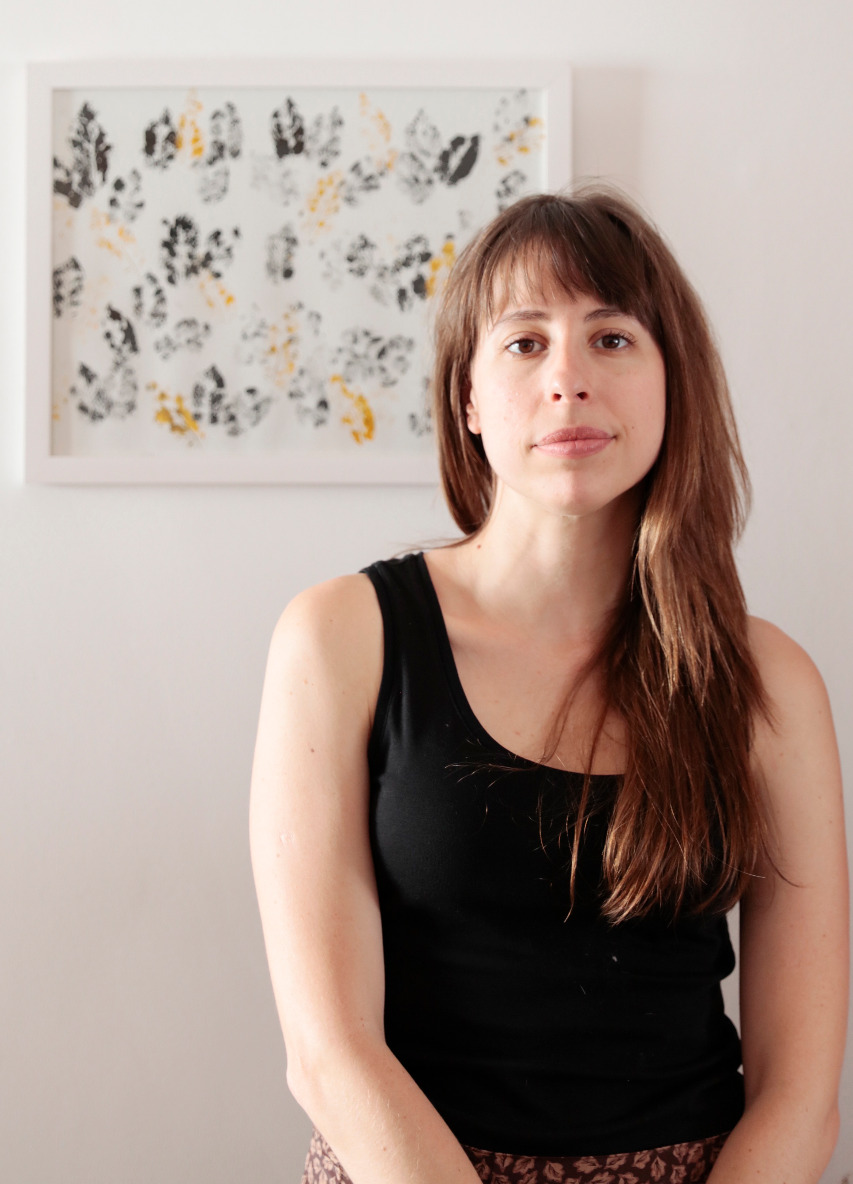
\includegraphics[width=\marginparwidth]{./images/PNLD2022-016-03.png}\\
A ilustradora Marina Magalhães (Arquivo pessoal)}

\paragraph{Publicações}
A autora tem publicações relacionadas aos povos indígenas no meio acadêmico como ``Gradação da omnipredicatividade na família Tupi-Guarani.'' (\textsc{forma y funcion}, 2019.) e ``A gramaticalização de verbos em partículas na língua Guajá e sua relação com a omnipredicatividade.'' (\textsc{boletim do museu paraense emilio goeldi}, 2019.)



\paragraph{Currículo}
Possui graduação em Letras Português - Licenciatura pela Universidade de Brasília (1999), mestrado em Linguística pela Universidade de Brasília (2002), doutorado em Lingüística pela Universidade de Brasília (2007), pós-doutorado em linguística pelo Centre National de la Recherche Scientifique (\textsc{cnrs}), Paris, França, sob a supervisão do prof. Dr. Francesc Queixalós (2013) e pós-doutorado na Universidade do Texas em Austin (\textsc{eua}), sob a supervisão da profª. Dra. Patience Epps (2019), com bolsa de estudos da \textsc{fapdf}. 


\section{Sobre o gênero}

%55 caracteres
\paragraph{O gênero} O gênero deste livro é \textit{prescritivos}. 


%596 caracteres
\paragraph{Descrição} 
Textos do gênero prescritivo têm como característica principal instruir
o leitor. Extremamente comuns na vida quotidiana, eles estão presentes
sempre que se precisa de uma guia ou uma orientação. São estruturas 
que oferecem padrões: leis, que podem ser jurídicas, como um código
penal, ou gramaticais, como um dicionário ou uma gramática; a constituição
de um país etc. Seu conteúdo é, de alguma forma, imutável, ao menos até que seja
mudado. O significado de uma palavra no dicionário deve continuar o mesmo
até que um novo seja adicionado. Enquanto isso, o texto
estabelecido será aquele que tem valor absoluto.


%603 caracteres
\paragraph{Interação} 
Ainda que não sejam os gêneros privilegiados pela literatura
como as narrativas ou os poemas líricos, os textos prescritivos
têm uma grande importância para a vida em sociedade. A todo 
tempo estamos recorrendo a estas obras, em geral de consulta, para
sabermos como devemos agir, seja uma dúvida a respeito da ortografia ou 
dos significados de uma palavra, seja a respeito de um direito ou dever
enquanto cidadão. É de extrema importância, portanto, que as crianças
sejam o mais cedo apresentadas a este gênero, ainda que com a 
devida abordagem lúdica que a idade demanda. 

\Image{No gênero prescritivo, o principal objetivo é instruir o leitor -- assim como a orientação de um dicionário. (Piqsels; Domínio público)}{PNLD2022-016-07.png}

%862 caracteres
\paragraph{Competências} 
As competências trabalhadas numa obra do gênero prescritivo como o 
\emph{Awa rapea} são diversas. 
Primeiro, há uma apresentação à necessidade de se fazer as coisas de um 
determinado jeito. É o mundo das regras e convenções sociais: há um modo 
convencionadamente correto de se escrever as palavras. E a partir de letras 
se formam palavras, que representam coisas. Então temos outra competência, 
que é a descoberta de novos vocabulários. Mesmo que alguns desses objetos já 
fizessem parte do imaginário de algumas crianças, agoras eles passam
a ser associados a suas representações escritas, o que corrobora numa complexificação
da realidade a partir deste novo universo. Ainda que pareça ser um gênero
limitante, são os conhecimentos fixados nestas obras que permitem a expansão
da criatividade com a garantia de que o outro irá entender já que as convenções são comuns.

\section{Temas}

\subsection{Quotidiano de crianças nas escolas; nas famílias e nas comunidades (urbanas e rurais)}

%136 caracteres
\paragraph{Abordagem} 
São apresentados os elementos que fazem parte do dia a dia de uma criança na comunidade indígena.
%206 caracteres
\paragraph{Descrição} 
A cada página, o aluno conhecerá algumas palavras da língua Awá-Guajá, junto à tradução em português
e uma ilustração em aquarela da mesma. Membros da comunidade, fauna e flora locais e demais questões
quotidianas são apresentadas ao aluno.
%275 caracteres
\paragraph{Competências} 
Este tema relaciona-se, principalmente, ao campo de experiência ``Espaços, tempos, quantidades, relações e transformações'',
descrito pela \textsc{bncc}, que tem como intuito instigar a investigação
do mundo natural e social, e brincar com elementos da natureza de diferentes culturas.


\section{Modelagem de aula}
A seguir você encontrará a descrição de uma aula modelo como exemplo 
prático de exploração do livro com estudantes. Esta seção apresentará 
orientações sobre como organizar a sala de aula para receber os 
estudantes, exercitar a interação verbal e prepará-los para o 
momento da leitura.

Em seguida, você encontrará a \textbf{Leitura dialogada}, um 
tópico destinado a te orientar para o momento específico da 
leitura com os estudantes. Por fim, no tópico 
\textbf{Propostas de atividades}, você encontrará ideias 
de práticas que pode explorar com as crianças em sala de 
aula após a leitura. 

Essas atividades podem ser trabalhadas de acordo com a 
disponibilidade do seu cronograma e fique à vontade para adaptá-las 
da forma que achar melhor para os seus estudantes. Cada turma é única 
e o seu conhecimento prático das características de cada aluno será 
essencial para definir a melhor forma de aplicar essas ideias. 

O objetivo deste manual é oferecer algumas ideias 
e inspirações para um trabalho que pode ser desenvolvido tanto 
a curto, quanto a médio e longo prazo. Sinta-se a vontade para 
personalizar a aula e torna-la sua, aplicando seus conhecimentos, sua 
personalidade e aproveite para fortalecer 
seu vínculo com a turma.


\subsection{Antes de ler}

\BNCC{EI03EO01} 
\BNCC{EI03EO02}
\BNCC{EI03EO03}
\BNCC{EI03EO07}
\BNCC{EI03CG01}
\BNCC{EI03CG02}
\BNCC{EI03CG03}

%Alterar o nível escolar nesse parágrafo.
Como este trabalho será realizado com crianças da \textbf{Pré-escola}, 
que ainda não têm muita intimidade com o livro enquanto objeto, você terá o 
papel de mediar este contato. 

Nosso objetivo é que os próprios estudantes possam manusear 
e explorar o livro de forma autônoma, mas, para que isto aconteça, você 
pode ajudar a tornar o caminho mais convidativo com atividades que tenham 
intencionalidade educativa. 

A \textsc{bncc} define intencionalidade educativa como ``organização 
e proposição, pelo educador, de experiências que permitam às crianças 
conhecer a si e ao outro e de conhecer e compreender as relações com a 
natureza, com a cultura e com a produção científica, que se traduzem nas 
práticas de cuidados pessoais (alimentar-se, vestir-se, higienizar-se), 
nas brincadeiras, nas experimentações com materiais 
variados, na aproximação com a literatura e no encontro com as 
pessoas''.\footnote{\textsc{bncc}, página 39}

É importante manter essa intencionalidade em mente não apenas na condução 
das atividades propostas neste manual, mas também para aproveitar as 
oportunidades espontâneas de construir conhecimentos que podem surgir durante 
a interação direta com os estudantes.

\begin{enumerate}
%836 caracteres
\item \textbf{O ambiente}\quad Antes de iniciar o trabalho com o livro, é importante que você 
prepare o ambiente para receber a turma. Como o trabalho com o livro terá 
três momentos (antes, durante e depois da leitura), seria interessante que você 
criasse um ambiente para cada etapa. Nas \textbf{Sugestões de referências complementares} 
você encontrará um artigo que discorre sobre a importância da organização da sala 
de aula para a educação infantil, que pode ser um bom guia para a criação desses 
ambientes. Para o momento antes da leitura, coloque para tocar o album de cantos 
guarani indicado nas leituras complementares. Ainda que não seja o mesmo povo
indígena que será trabalhado, ainda assim a língua dos Guarani pertence ao mesmo tronco
linguístico dos Awá-Guajá, então servirá como introdução à cultura deste povo.

\Image{As crianças guarani da aldeia Tenondé Porã podem ser uma referência para a atividade. (Ian Pozzobon; CC BY-NC-SA 2.0)}{PNLD2022-016-09.png}

%413 caracteres
\item \textbf{Materiais}\quad Um aparelho de som, um projetor, urucum, 
faixas de panos e colares. 

Quando os estudantes estiverem na sala,
peça que eles se disponham pelo espaço e coloque a música. Caso eles não 
se movimentem, você pode dançar no ritmo para incentivá-los. A ideia é que
conforme um comece, os outros vão repetindo. Chame a atenção para os movimentos
que eles fizerem, peça aos outros para olharem, e elogie, pedindo que todos
o imitem. Faça isso até que todos tenham tido um momento de atenção especial. 


\item \textbf{Desenvolvimento}\quad Com a música tocando ao fundo, mostre
às crianças a capa do album. Lá, elas verão crianças da etnia Guarani
enfeitadas para uma festividade de seu povo. Eles têm penas e colares no
pescoço, uma faixa na cabeça, e tinta vermelha no rosto. Disponha esses 
elementos para as crianças e peça que eles, com seu auxílio, tentem
ficar parecidos com o que veem na imagem, que pode estar projetada num telão. 
Para a tinta, o urucum pode ser utilizado, visto que é um pigmento natural
e não oferece risco à saúde das crianças.
Depois da aparência, é a hora de movimentar o corpo conforme a música.
Quando as crianças estiverem prontas, peça que elas se disponham pelo espaço. 
Caso eles não se movimentem, você pode dançar no ritmo para incentivá-los. A ideia é que
conforme um comece, os outros vão repetindo. Chame a atenção para os movimentos
que eles fizerem, peça aos outros para olharem, e elogie, pedindo que todos
o imitem. Faça isso até que todos tenham tido um momento de atenção especial. 

\item \textbf{Perguntas para avaliar} Os alunos engajaram na proposta? 
Eles agiram sem muito estranhamento aos novos costumes que estavam sendo apresentados?
Eles fizeram perguntas e comentários a respeito dos povos indígenas?
\end{enumerate}

\subsubsection{A interação verbal} 
Criar situações em que as crianças precisam dialogar diretamente com 
você é uma das práticas mais importantes de Literacia, pois elas estimulam 
o desenvolvimento linguístico, ampliam o vocabulário e reforçam a 
capacidade dos estudantes de compreenderem o que ouvem e se expressarem 
pela fala. O diálogo livre com a criança também reforça sua autoestima, pois 
a faz se sentir ouvida e valorizada pelo adulto, ao vê-lo prestar atenção 
no que ela tem a dizer. Portanto, sempre que possível, reserve um tempo na 
aula apenas para a interação verbal. 

Como esse tipo de interação é espontânea e intimamente atrelada ao 
desenvolvimento de cada estudante, nossas orientações não serão específicas. 
A ideia é que você adapte este momento de acordo com as respostas e os 
repertórios das crianças. É um momento de estreitamento de vínculos e, portanto, 
fique a vontade para ser espontânea e para explorar os tópicos que achar 
mais interessantes para a sua turma.

Inicie as conversas com naturalidade. Você pode partir de comentários
sobre as atividades, sobre um som, um movimento. Você deve incentivá-los a 
se expressar.

Fique atento a todas as formas de expressão: os gestos, as falas, as 
expressões faciais, para onde olham\ldots{} tudo pode ser explorado durante a conversa. 
Demonstre curiosidade sobre eles, seja um ouvinte entusiasmado e incentive que eles 
conversem entre si. Faça perguntas e construa a resposta junto com as crianças, 
a partir dos sons que eles emitem ou de informações que você saiba. 

A seguir, algumas dicas que podem contribuir para que a interação verbal 
seja produtiva em sua sala de aula: 

\begin{enumerate}
\item Sente-se no chão e brinque com eles, estabelecendo 
contato visual. Embora não consigam falar, vocalizações, 
gestos e expressões faciais podem ser boas formas de comunicar.

\item Não se esqueça que a conversa é uma troca e, portanto, 
evite ficar falando sozinho ou desvalorizar as respostas dos 
bebês porque não são palavras completamente articuladas. 
Nunca descarte uma tentativa de comunicação. 

\item Evite utilizar falas negativas que desencorajam o diálogo. 
Se precisar que a turma corrija algum comportamento, explique 
claramente a razão e oriente com calma. Incentive positivamente 
as crianças e destaque o motivo de seus elogios. 

\item Aproveite alguns momentos durante a conversa para chamar 
a atenção das crianças para os sons das palavras e das letras que você 
acabou de usar ou que eles pronunciaram.  

\item Fale sempre com as crianças, pois, apesar de cometerem alguns erros
ou estarem começando a falar, são capazes de compreender muito.

\item Explore possibilidades de interação como apontar e 
nomear objetos, pessoas e animais, imitar a criança ou pedir que 
ele o imite, fazer caretas, jogar beijos, reproduzir sons de 
animais para que repitam, ensinar os nomes de partes do corpo, 
entre outras atitudes que estimulem a comunicação com a criança. 

\item Muitas dessas dicas poderão ser aproveitadas pela 
família durante a prática da Literacia Familiar. Portanto, 
se achar necessário, compartilhe algumas destas orientações 
com as famílias dos estudantes.
\end{enumerate}


\subsection{A leitura dialogada}
Este é o momento em que será realizada a leitura propriamente dita. 
Se possível, crie um \textit{cantinho da leitura} em sua sala de aula. Um 
ambiente confortável, de preferência em que todos se sentem no chão ou 
em pufes para que consigam enxergar as ilustrações do livro que está 
sendo lido e interagir com facilidade. Se houver possibilidade, mantenha 
sempre os livros da turma em uma altura da estante que permita fácil 
acesso para os estudantes ou guarde os livros em uma caixa que as crianças 
possam mexer com autonomia. É importante que elas tenham autonomia para 
acessar os livros e se sintam à vontade para pegá-los sempre que quiserem. 

\Image{É importante que o cantinho da leitura proporcione autonomia para as crianças. (Elza Fiúza/ Agência Brasil; CC BY-NC 2.0)}{PNLD2022-016-08.png}

Outra possibilidade de ambiente para esta leitura, se a escola permitir, 
é efetuar essa leitura ao ar livre, embaixo de uma árvore, onde as crianças 
possam ouvir os sons dos pássaros e sentir o cheiro da grama. Sair da sala 
de aula pode oferecer um ótimo leque de experiências aos seus estudantes e 
reforçar a conexão entre a natureza do livro e a realidade.  

Reserve uma boa parte da aula para o momento da leitura com os estudantes, 
pois é importante que esse momento aconteça sem pressa. O objetivo da 
leitura dialogada é que seja uma leitura em bate-papo. A criança deve 
assumir um papel ativo na leitura, mesmo que ainda não seja capaz de 
ler sozinha. Além de promover o gosto pela leitura, esta prática estimula 
o desenvolvimento da linguagem, enriquece o vocabulário e 
aumenta o conhecimento de mundo.

%Especificar o livro.
No caso de ``Awa rapea'' o diálogo durante a leitura é 
ainda mais importante, considerando que há palavras numa língua que não é o português. 
Você deve interagir com eles durante toda a 
leitura, servindo de base para a pronúncia das palavras em Awá-Guajá.
Para isso, utilize o guia de pronunciação que se encontra ao final do livro.

A seguir, algumas orientações para aproveitar este momento: 

\begin{enumerate}
%177 caracteres
\item \textbf{Como começar}\quad Sente-se em um lugar acessível, 
onde todos conseguirão ouvir bem a sua leitura e enxergar as ilustrações 
quando você estiver mostrando o livro ou eles estiverem manuseando-o. 
Antes de abrir o livro, chame a atenção dos estudantes para a capa. 
Faça perguntas sobre a capa, como: 

\begin{itemize}
\item Que lugar é este?
\item Quem já foi na floresta?
\item O que tem na floresta?
\item Onde mais os indígenas moram?
\end{itemize}

Estas perguntas te ajudarão a avaliar repertório das crianças. 
Não há problema se as perguntas que você fizer não forem respondidas pelos 
estudantes. Você mesma pode respondê-las de forma simples e articulada. Se achar 
conveniente, peça que repitam algumas palavras com você e valorize tentativas 
de imitar a sua fala. 

%230 caracteres
\item \textbf{Manuseio}\quad Deixe que as crianças manuseiem o livro 
e explore com elas todos os elementos que o compõe. Mostre o que é a 
capa e onde estão as páginas. Leia o título do livro em voz alta, seguindo 
a leitura com o dedo, indicando as letras. 

%495 caracteres
\item \textbf{Diálogo}\quad A cada página ou a cada nova palavra,
chame a atenção dos alunos para ele. Como se trata de uma língua estrangeira, 
apoiada no manual fonético ao fim do livro, chame a atenção às palavras na língua 
indígena. Faça perguntas como:

\begin{itemize}
\item O que é isso?
\item Vocês já viram alguma vez? 
\item Onde eles ficam? 
\end{itemize}

Se os estudantes não conseguirem responder, explique ou mostre uma 
imagem ou um vídeo. Traga referências além da ilustração e da frase. 
Incentive-os a relatar experiências com esses objetos.

%346 caracteres
\item \textbf{Escuta}\quad Elogie atitudes positivas, como 
tentar tomar o papel central na leitura. Se os estudantes tentarem 
tomar o seu lugar e começar a narrar a história --- com palavras já articuladas 
ou não --- valorize e escute com atenção o que estiverem falando. Mas não 
force a leitura. Se as crianças estiverem cansadas, faça outra atividade 
e retorne depois. 

\includepdf[nup=2x3, 				% grid
			%offset=-15mm -5mm, 	% posição
			scale=.8, 				% tamanho da página
            delta=4mm 4mm, 			
            frame,
            pages={4-5,14-15,30-31}]{./pdfs/\jobname_MIOLO.pdf}

%935 caracteres
\item \textbf{Leitura}\quad Faça perguntas e comentários que aumentem o 
interesse e aticem a curiosidade das crianças sobre a história. Leia 
as palavras em Awá-Guajá e peça que eles repitam. Auxilie os que tiverem
mais dificuldade com a pronúncia. Então faça perguntas sobre as palavras
para que eles respondam:

\begin{itemize}
\item Como se diz céu?
\item E terra?
\item Como se diz mata?
\end{itemize}

Não tenha pressa em passar as páginas. Como são muitas palavras novas,
numa língua que eles não conhecem, selecione um pequeno número para
trabalhar. 

Não deixe que eles fiquem sem entender do que se trata. Crie 
um ambiente amigável onde a criança se sinta à vontade para fazer 
perguntas e comentários durante a leitura.


%382 caracteres
\item \textbf{Interação}\quad Nomeie os elementos das ilustrações 
do livro, apontando para elas com o dedo. Destaque os sons de algumas 
palavras. Interrompa a leitura em alguns momentos e peça que 
os estudantes repitam palavras, como \textit{kwarahy}, \textit{amỹna}, \textit{iwa}. Se possível, 
leia a mesma palavra e sua tradução várias vezes.
\end{enumerate}


\subsection{Proposta de atividade 1}

\BNCC{EI03EF03} 
\BNCC{EI03EF04} 
\BNCC{EI03EF07} 
\BNCC{EI03ET05} 
\BNCC{EI03ET01} 
 

\begin{enumerate}
%700 caracteres
\item \textbf{Contexto}\quad Após a leitura dialogada, é hora de criar 
atividades que proporcionem aos estudantes experiências novas a partir do livro
que acabaram de conhecer. Nesta idade é fundamental explorar os sentidos da criança e 
ajudá-lo a experimentar os conhecimentos que acabaram de conhecer de formas diversas. Se achar 
conveniente, convide os estudantes a se sentarem em roda no chão.

\item \textbf{Materiais}\quad Papeis para escrever e imagens impressas ou desenhadas, de preferência
em papel cartão.

%650 caracteres
\item \textbf{Ambiente}\quad 
Pergunte se as crianças já brincaram de jogo da memória. Então, repasse as regras e o funcionamento
do jogo. As duas partes a serem achadas são: o nome em Awá-Guajá, e uma ilustração de 
seu significado. Por exemplo, ``iwá'' forma par com uma imagem de um céu, ``wya'', com uma imagem da terra,
e assim por diante. Repassem em frente à turma todos os nomes e todas as imagens que farão parte do jogo.
Deixe alguns de fora para não ficar tão difícil. Forme os pares e deixe que todos vejam. 
Para que a dinâmica seja um pouco mais organizada, a depender do tamanho da turma, peça
que formem pequenos grupos. Neste caso, não devem ser muitos, para que você não perca muito
a atenção sobre eles. 

%950 caracteres
\item \textbf{Atividade}\quad 
Quando já estiverem todos dispostos no chão com os cartões, comece o jogo. 
Quando um cartão com uma palavra for virado, quem levantou deve tentar ler o que está escrito.
Para isso, você deve ajudar, já que eles ainda estão em fase de apresentãção à leitura.
Mas é importante que eles sejam incentivados ainda assim. 


%550 caracteres
\item \textbf{Interação}\quad O livro pode e deve ser 
manipulado pelos estudantes. Incentive que eles folheiem as páginas afim de encontrar a palavra 
escrita no cartão, ou a imagem correspondente a ela. 


\item \textbf{Perguntas para avaliar}\quad
Os alunos sentiram-se à vontade para tentar ler as palavras em língua 
indígena? Eles engajaram de um modo geral na atividade? 
HOuveram ao menos alguns acertos nas formação dos pares? 


\end{enumerate}
\subsection{Proposta de atividade 2}

\begin{enumerate}
%700 caracteres
\item \textbf{Contexto}\quad 
Após a leitura dialogada, é hora de criar 
atividades que proporcionem aos estudantes experiências novas a partir do livro
que acabaram de conhecer. Nesta idade é fundamental explorar os sentidos da criança e 
ajudá-lo a experimentar os conhecimentos que acabaram de conhecer de formas diversas. 
Informe aos alunos que eles vão para a área externa da escola para fazer uma brincadeira. 

\item \textbf{Materiais}\quad
Papeis com adesivo e caneta para escrever.

%650 caracteres
\item \textbf{O ambiente}\quad 
As crianças devem ser levadas para a área externa da escola, ou 
a área de lazer, se for possível. De preferência um lugar onde tenha 
muitos objetos diferentes, em alguma medida similares aos que foram 
apresentados no livro. Utilizando os mesmos papeis da atividade anterior ou refazendo-os,
expalheo-os pela escola. De preferência, faça mais dois ou três de cada um.

%950 caracteres
\item \textbf{A atividade}\quad 
As crianças terão como missão encontrar os papeis com as palavras escritas 
e trazê-los de volta a um lugar previamente combinado. Faça mais de um 
papel para o mesmo objeto para que mais de um grupo ou pessoa o encontre e 
a brincadeira dure um pouco mais. Este tipo de atividade demanda atividade física. 
As crianças irão correr à procura dos papeis nos mais diversos lugares, então 
peça para que tomem cuidado para não cair nem machucar umas às outras. 
Caso eles estejam com dificuldade de encontrar, dê dicas utilizando 
os textos finais livro que dão informações sobre a cultura Awá-Guajá, por exemplo: 

\begin{itemize}
\item É o lugar onde os Awá-Guajá descansam!
\item É o lugar onde os Awá-Guajá se reunem para estudar!
\end{itemize}

%550 caracteres
\item \textbf{Interação}\quad O livro pode e deve ser 
manipulado pelos estudantes. Durante toda a brincadeira 
o livro pode ser consultado para olhar as imagens e os 
nomes das coisas. Uma das crianças pode ficar responsável
por consultar as informações no livro enquanto as outras correm
atrás dos papeis. No entanto, é importante que esta função não
seja fixa, e que todos possam trocar de postos.


\item \textbf{Perguntas para avaliar}\quad
Os estudantes se engajaram na atividade? Conseguiram associar os nomes na
língua indígena às coisas física de seu quotidiano?
Conseguiram trabalhar em pequenos grupos? 

\end{enumerate}

\section{Literacia familiar}
O \textsc{pna} dá destaque especial para a importância do envolvimento da família 
no processo pedagógico nesta faixa etária e denomina Literacia Familiar o conjunto 
de experiências e práticas relacionadas à linguagem (oral, escrita ou lida) vivenciadas 
com os cuidadores. 

Essas estratégias podem começar a ser colocadas em prática desde a 
gestação e continuar até o final da adolescência. São práticas simples e divertidas 
que estimulam o desenvolvimento de quatro atividades fundamentais: ouvir, falar, 
ler e escrever que criam momentos de afeto e interação para a família. 

Para que esse trabalho conjunto entre escola e família funcione, é 
fundamental que a escola esteja em constante diálogo com os responsáveis e 
você consiga orientá-los. Um grupo em aplicativos de mensagens instantâneas ou um 
grupo de e-mails são saídas viáveis para que a comunicação se estabeleça e pode ser 
uma forma útil das famílias compartilharem suas vivências e trocarem sugestões 
de abordagens, sempre contando com a sua mediação. 

Com o objetivo de incentivar 
a prática da \textit{literacia familiar}, se possível, organize um rodízio entre os familiares 
das crianças para emprestar o livro da biblioteca da turma. Neste caso, crie um caderno 
de registro e estabeleça períodos para cada família ficar com o livro. É importante 
que os familiares compreendam a seriedade deste compromisso, pois o livro pertence 
ao acervo da sala e, portanto, deve ser bem cuidado e devolvido na data acordada. 

Se não for possível garantir o acesso direto dos cuidadores da criança ao livro, 
grave um vídeo direcionado a eles, contando a história e apresentando algumas 
das ilustrações. O importante é que os familiares saibam com clareza qual livro 
está sendo trabalhado, a história contada e se sinta seguro para explorar as temáticas 
do livro com a criança. Orientações claras e a manutenção do canal de comunicação com 
os responsáveis é essencial para que eles se sintam seguros e à vontade para fazer perguntas 
se tiverem dúvidas. 

Neste manual, você encontrará algumas práticas que podem ser 
recomendadas aos familiares para ajudá-los a expandir e aprofundar o trabalho 
que você iniciou em sala de aula.


\subsection{Importância da leitura}
Na escola, aprendemos a ler letras, mas é importante ter em mente que nós 
lemos o mundo desde muito pequenos: “lemos” os animais que passam pelos nossos 
quintais, a expressão no rosto dos nossos familiares, as cores que pintam o céu 
em um fim de tarde. 

Vamos aprendendo, ao longo da vida, a interpretar acontecimentos 
e sons que escutamos e a utilizá-los para nossa comunicação. Aprender a ler textos e 
escrevê-los expande a nossa leitura do mundo, pois permite que sejamos capazes de 
interpretar um código e experimentar, a partir dele, novas experiências e conhecimentos. 

O simples contato com os livros já permite um leque grande de sensações: 
sentimos as texturas, as formas, vemos as cores do livro, escutamos o som da página 
virando e o som da voz do narrador, se a história estiver sendo lida em voz alta. Para um 
bebê, são experiências que podem contribuir diretamente com o desenvolvimento psicomotor 
e cognitivo. 

Nosso papel, enquanto mediadores de leitura, é contribuir para que essas 
sensações sejam associadas a momentos positivos, de construção de 
conhecimento e exercício de imaginação. 

Com os livros, podemos conhecer mais da história humana, descobrir informações 
novas sobre sociedades diferentes da nossa, imaginar situações e contextos inéditos 
para nós e aumentar o nosso repertório. São por meio deles que melhoramos nossa 
capacidade de interpretação, de expressão, de análise e senso crítico. Boas habilidades 
leitoras podem contribuir para o desenvolvimento de um estudante em todas as outras 
disciplinas, pois exercem influência direta na forma como absorvemos e 
construímos conhecimento.


\subsection{O papel da família na formação do leitor}
A família é peça fundamental na formação do leitor, pois é ela quem primeiro 
ensina a criança a ler. Não apenas os textos escritos, mas a ler o mundo, a 
interpretar os estímulos que a cercam, a construir seu próprio vocabulário e a 
comunicar seus pensamentos e necessidades. Na fase em que estão, os bebês 
absorvem o conhecimento com voracidade e tentam aprender a se comunicar. 

O universo das letras é muito presente na vida das crianças antes mesmo de sua 
entrada na escola. Aparece nas histórias e ilustrações do livro que o cuidador 
lê ao colocá-la para dormir, nas situações em que vê os responsáveis se comunicarem 
pela escrita ou nos textos que podem permear seu cotidiano (nos outdoors, na 
televisão, no celular, manuais de instrução entre outros). 

Os familiares têm, 
portanto, uma ótima oportunidade de apresentar a leitura com leveza, de forma 
prazerosa, associado ao contexto em que a criança vive e à momentos de diversão. 
Você poderá orientar os pais nesta tarefa, ensinando-os com este guia a aproveitar 
as oportunidades para trabalhar a Literacia com a criança.


\subsubsection{Práticas de literacia familiar} 

São muitas as experiências que a prática da \textit{literacia familiar} 
pode oferecer às crianças. A seguir, explicamos cada uma delas para que você possa, 
se achar necessário, compartilhar com os responsáveis enquanto estiver orientando-os: 

\paragraph{Interação verbal} Aumentar a quantidade de conversas com as 
crianças, fazendo perguntas para incentivar o diálogo.

\paragraph{Leitura dialogada} Interagir com a criança durante a leitura 
em voz alta, criar expectativa sobre o livro, chamar a atenção para detalhes 
das ilustrações e comentar o enredo.

\paragraph{Narração de histórias} Interagir com a criança enquanto 
estiver narrando uma história, por exemplo, incluindo-a na ação, utilizando 
marionetes ou permitindo que ela complete a narrativa.

\paragraph{Contatos com a escrita} Apresentar as letras para as 
crianças, incentivar que tentem escrever ou ler, ajudá-los a desenhar letras, 
entre outras formas de incentivar o contato com as palavras.

\paragraph{Atividades diversas} Qualquer atividade com a criança 
pode ser utilizada para contribuir para a alfabetização. Jogos, brincadeiras, 
instrumentos musicais, canto, dança, passeios e viagens oferecem boas 
oportunidades de aprendizado.

\paragraph{Motivação} Atitudes que motivem as crianças à envolver-se com 
o mundo da leitura e da escrita.

\subsection{Exercitando a literacia familiar}

\BNCC{EI03ET03} 
\BNCC{EI03EF07} 
\BNCC{EI03EF08} 
\BNCC{EI03EF03} 
\BNCC{EI03EF05} 

\marginnote{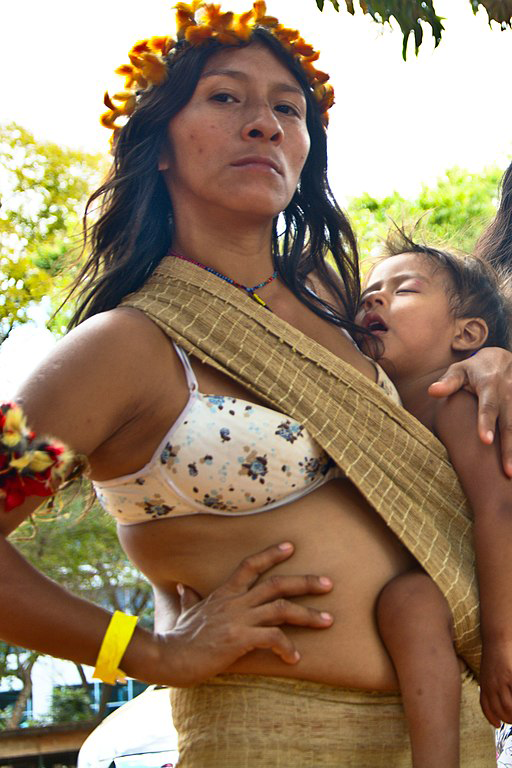
\includegraphics[width=\marginparwidth]{./images/PNLD2022-016-10.png}\\
Mulher Awá-Guajá na Marcha das Mulheres Indígenas (Apib comunicação; CC-BY-SA-2.0)}

\begin{enumerate}
%700 caracteres
\item \textbf{Como começar}\quad Como se trata de um trabalho com
uma língua estrangeira, instrua os pais a consultar o manual de 
pronúncia ao fim do livro. Será uma oportunidade para que eles
próprios conheçam mais a cultura do país onde vivem. Também no final do livro,
os pais e cuidadores encontrarão um índice informativo sobre a cultura deste povo.
Estes dados devem ajudá-los na hora da leitura com os pequenos caso estes 
façam perguntas sobre a vida destas pessoas. Se achar conveniente, compartilhe com 
os familiares algumas dicas das seções Interação verbal 
e Leitura dialogada e as indicações nas Referências Complementares 
para ajudá-los a explorar as possibilidades oferecidas pelo livro. 

%650 caracteres
\item \textbf{Leitura}\quad A família pode continuar 
explorando os temas apresentados pelo livro. Os familiares podem explorar 
elementos do cotidiano que se relacionam à história e indicar a conexão 
entre o que viram na ilustração e suas realidade. ``Awa rapea'' apresenta 
o quotidiano de pessoas que moram numa comunidade indígenas, num ambiente rural,
com características específicas. Os adultos podem, a cada nova informação, comparar
a realidade que estão aprendendo com a que a criança vive, com o cuidado
de não instaurar nisso nenhum julgamento de valor, mas sim de descoberta
do diferente. Oriente-os a mostrar os elementos descritos no livro como ``céu'',
``árvore'', ``rede'' na realidade de suas casas, e utilizar estes elementos para 
relembrar a história do livro. Se houver possibilidade, eles podem pesquisar 
imagens de outros povos indígenas que tenham elementos similares e assim os relacionar à pintura da autora. 

%1073 caracteres
\item \textbf{Instrução}\quad Buscando incentivar a interação das crianças
com outras pessoas de seu entorno, instrua os pais a entregar o livro para a criança 
e pedir que ela explique palavras ou informações sobre o povo Awá-Guajá para outro familiar, vizinho ou amigo. 
Mesmo que as informações não pareçam 
completas para o adulto, é importante que ele ouça com atenção e 
valorize todas as tentativas da criança. Afinal, ao tentar explicar, 
ela manipulará o livro, treinará a coordenação motora, conhecerá as texturas 
do objeto e poderá imitar a forma como o adulto 
conta as explica, treinando a fala. 
\end{enumerate}

 
\section{Sugestões de referências complementares}

\subsection{Livros} 

\begin{itemize}
\item LINS, Guto. Livro infantil? projeto gráfico, metodologia, subjetividade. São Paulo: Rosari, 2002.
Livro que aborda a importância das escolhas visuais (ilustração, projeto gráfico, lettering) na literatura infantil.  

\item HUNT, Peter. Crítica, teoria e literatura infantil. São Paulo: Cosac Naify, 2010.
Livro sobre crítica de literatura infantil que contêm definições de livro ilustrado e livro imagem. 
\end{itemize}

\subsection{Artigos}

\begin{itemize}
	\item \textsc{bonin}, Iara Tatiana. \emph{Encarte Pedagógico \textsc{i}. Culturas indígenas na sala de aula}.
	Publicação do Conselho Indigenista Missionário (Cimi), jan/fev 2015. Disponível em: \url{https://cimi.org.br/wp-content/uploads/2020/01/Porantim372_JanFev_Encarte-2015.pdf}. Acesso em 27 ago. 2021.
	Artigo científico destinado a profissionais da educação com informações que ajudam a desmistificar informações
	acerca dos povos indígenas brasileiros com a apresentação de dados e referências que podem ser utilizados em sala de aula.
	\item \textsc{sardelich}, Maria Emilia. \emph{Leitura de Imagens, Cultura Visual e Prática Educativa.} 
In: Cadernos de Pesquisa. V.36, n.128, p.451-472, mai/ago.2006. Disponível em: \url{https://www.scielo.br/pdf/cp/v36n128/v36n128a09}. 
Acesso em 29 abr 2021. 
Artigo acadêmico que discorre sobre a importância de trabalhar cultura 
visual na educação na sociedade contemporânea. 

\item \textsc{pranke}, Marha Elfrida. \emph{Organização dos espaços da sala de aula na Educação Infantil.} Disponível em: 
\url{http://centraldeinteligenciaacademica.blogspot.com/2016/04/organizacao-dos-espacos-da-sala-de-aula.html}. Acesso em 04 mai 2021. 
Artigo acadêmico que discorre sobre a importância da rotina e de criar ambientes dentro da sala de aula na Educação Infantil.  
\end{itemize}

\subsection{\textit{Sites}}

\begin{itemize}
\item Vídeos “Conta pra mim” no site do PNA. Disponível em: \url{http://alfabetizacao.mec.gov.br/contapramim}. 
Acesso em 13 abr. de 2021.
Página do MEC com vídeos sobre leitura dialogada que visam incentivar a Literacia Familiar. Muitas das 
técnicas, explicações e materiais disponíveis nessa página podem ser utilizados em aula, mas o site também 
pode ser uma ótima indicação para ajudar a direcionar os cuidadores dos estudantes a praticar 
a literacia familiar e leitura dialogada.

\item Vídeo “Livros de imagem: como utilizar com as crianças?” do canal Conta Outra. Disponível em Youtube. 
Acesso em 14 abr. 2021. 
Neste vídeo, a pedagoga Bel explica o que são livros de imagem e faz sugestões para mediar a leitura com 
crianças. Se você achar conveniente, esse vídeo pode ser recomendado aos familiares da criança 
para inspirá-los na leitura dialogada. 

\end{itemize}

\subsection{Para os estudantes}
\begin{itemize}

\item Album de música do povo Guarani realizada pelo grupo Memória Viva Guarani,
``Ñande Reko Arandu''. Disponível em Youtube. Acesso em 23 ago. 2021. 
As quinze faixas do album são cantadas em idioma guarani, do mesmo tronco 
linguístico que a língua dos Awá-Guajá. É uma outra forma de aproximar 
os estudantes da cultura dos povos indígenas brasileiros. 


\end{itemize}


\section{Bibliografia comentada}

\subsection{Livros}

\begin{itemize}
\item \textsc{brasil}. Ministério da Educação. Base Nacional Comum Curricular. Brasília, 2018.
Consultar a BNCC é essencial para criar atividades para a turma. Além de especificar 
quais habilidades precisam ser desenvolvidas em cada ano, é fonte de informações sobre 
o processo de aprendizagem infantil. 

\item \textsc{brasil}. Ministério da Educação. Secretaria de Alfabetização. Conta pra mim: Guia de Literacia Familiar. 
Brasília: MEC, SEALF, 2019. Disponível em: \url{http://alfabetizacao.mec.gov.br/images/conta-pra-mim/conta-pra-mim-literacia.pdf}
Este guia é voltado aos pais e oferece explicações em uma linguagem bastante acessível e detalhada as práticas de Literacia Familiar, 
como praticar leitura dialogada, como narrar histórias, como exercitar interação oral, formas de proporcionar contatos com a escrita à criança etc. 
 
\item \textsc{brasil}. Ministério da Educação. Secretaria de Alfabetização. PNA Política Nacional de Alfabetização/Secretaria 
de Alfabetização. Brasília: MEC, SEALF, 2019.
Um guia fundamental para trabalhar pré-alfabetização e alfabetização de estudantes, que ressalta a importância da Literacia e da Numeracia. 


\end{itemize}

\subsection{Artigos}

\begin{itemize}
\item \textsc{costa}, A. C. C.; \textsc{santos netos}, J. A.; \textsc{bortolin}, S; \textsc{pereira}, Ana Paula. O livro de imagem e a mediação na escola. 
In \textsc{vii secin}, Universidade de Londrina. Disponível em \url{http://www.uel.br/eventos/cinf/index.php/secin2017/secin2107/paper/viewFile/445/296}. 
Acesso em 29 abr 2021. 
Esse artigo reflete sobre a importância de se apresentar livros de imagem para os estudantes na escola para que as crianças aprendam a ler imagens. 

\item \textsc{nannini}, P. B. R.; \textsc{medeiros}, J. P. S.; \textsc{ribeiro}, J. M. Leitura em cena: Vivências em sala de aula com livro de imagens. 
Literartes, n. 3, p. 82-101, 2014. DOI: 10.11606/issn.2316-9826.literartes.2014.89204. 
Disponível em \url{https://www.revistas.usp.br/literartes/article/view/89204/92115}. Acesso em 29 abr. 2021. 
Artigo acadêmico sobre um trabalho utilizando o mesmo livro de imagem com crianças da educação infantil e ensino médio. 
É uma forma interessante de perceber que a leitura de imagens pode ser explorada com qualquer faixa etária. 
\end{itemize}

% \includepdf[nup=2x2, 					% grid
			% offset=-15mm -5mm, 		% posição
			% scale=.8, 				% tamanho da página
            % delta=4mm 4mm, 			
            % frame,
            % pages={1-4}]{pdfs/PNLD2022-016_MIOLO.pdf}

\end{document}
